\chapter{Syntax-Driven Verification} % compare to CFG-driven
\section{Introduction}
While the methodology presented in the previous chapter
for verifying memory preservation works well, it is not ideal.
\index{memory!preservation}
The need to manually formulate regions
and the amount of work required for developing invariants reduces potential scalability.
\index{scalability}

To build on the work from the previous chapter,
this chapter introduces the concept of \emph{\acp{fmuc}}
\index{certificate}
generated by untrusted, informal tools.
\Acp{fmuc} consist of two main components:
theorems on memory usage and \emph{proof ingredients}.
\index{proof!ingredients}
The proof ingredients are assumptions on memory layout,
control flow information, and invariants
generated to reduce the amount of work required from end users.
Information on how these certificates are generated can be found in \cref{se:fmuc_gen}.
This includes the algorithm for control flow information extraction
as well as how symbolic execution is used
to produce the preconditions and proof ingredients.
\index{symbolic execution}

Once generation is complete, the certificate and the original assembly
can then be loaded into an interactive theorem prover.
In the theorem prover,
\index{theorem!prover}
minimal user input is required for discharging \iac{fmuc}'s lemmas and theorems
via the proof ingredients and customized proof strategies.
\index{proof!ingredient}
\index{proof!strategy}
A simple example demonstrating usage along with 
further information on the structure of \acp{fmuc} can be found in \cref{se:fmuc_ex}.

After going into further detail on \acp{fmuc} verification in \cref{se:fmuc_ver},
\cref{se:syntax_example} provides an example to illustrate the generation
and verification process.
On its own, that example could theoretically overwrite its own return address
due to its pointer arguments, causing \ac{cfi} issues.
The associated \ac{fmuc} provides preconditions to prevent such cases
along with a formal proof of return address preservation under those conditions. 

Following the more full example in \cref{se:syntax_example} is a full case study
on the Xen Project hypervisor~\citep{chisnall2008definitive} in \cref{se:xen}.
\index{Xen}
Unlike the HermitCore work in \cref{se:cfg_application},
\index{HermitCore}
no modifications were made to the Xen build process
and the basic utility \texttt{objdump} was used for disassembly.
In total, \acp{fmuc} were generated and proofs discharged in Isabelle
for 251 Xen functions.
Minimal user interaction was required;
on average, only \num{85} lines of additional proof were needed
for every \num{1000} assembly instructions verified.
In total, the \num{12252} assembly instructions
were verified with only \num{1047} manual proof lines added,
all of which were simple reuses of established proof methods.
The majority of added lines of proof involved guiding loop invariant application.

\section{Overview of \acsp*{fmuc}}\label{se:fmuc_ex}
\Cref{fig:fmuc} provides an example of \iac{fmuc}.
\Acp{fmuc} are produced from assembly code,
which may be generated by a disassembler such \texttt{objdump}, IDA\fturl{https://www.hex-rays.com/products/ida/index.shtml},
Ghidra's decompiler\fturl{https://ghidra-sre.org/}, or Capstone~\citep{capstone},
or generated directly by a compiler when source code is available.
Each function specified for verification receives \iac{fmuc};
those that are not included in the verification effort,
including system calls and functions from dynamic libraries,
can be treated as black boxes, the usage of which is described in \cref{sse:fmuc_comp}.

\begin{figure*}
  \centering
  \caption{Example \ac{fmuc}}\label{fig:fmuc}
\end{figure*}

\section{\acs*{fmuc} Generation}\label{se:fmuc_gen}
\begin{figure*}
  \centering
  \begin{tikzpicture}[>=stealth, gnode/.style={draw, rounded corners, text centered}]
    \graph[grow right=2.8cm]{
      Assembly[gnode] ->[dashed]
      "Control Flow Graph"[gnode, text width=1.4cm] ->["\ref{sse:cfg_extract}"]
      "Syntactic Control Flow"[gnode, text width=1.7cm] ->["\ref{sse:mem_reg}"]
      "Memory Regions and \acsp*{mrr}"[gnode, text width=1.5cm] ->["\ref{sse:inv_gen}"]
      Invariants[gnode] ->[dashed] Certificate[gnode];
    };
  \end{tikzpicture}
  \caption{FMUC Overview}\label{fig:overview}
\end{figure*}

The general procedure for generating \acp{fmuc}, laid out in \cref{fig:overview},
can be broken up into three main parts.
The first part involves control flow extraction from assembly using \iac{cfg} analysis
similar to angr's CFGFast~\citep{shoshitaishvili2016state},
\index{angr!CFGFast}
ultimately producing \iac{scf} (details of which are presented
in \cref{sse:cfg_extract}).
Afterwards, per-basic block symbolic execution,
\index{basic block}
\index{symbolic!execution}
as detailed in \cref{ch:symbolic_execution},
is utilized to generate the set of memory regions
\index{memory!region}
read and written by the function in question.
To eliminate duplicates and produce \acp{mrr}
showing which regions overlap or are enclosed or separate,
the region sets are fed to the \ac{smt} solver Z3~\citep{de2008z3}
as described in \cref{sse:mem_reg}.
% TODO: may not need the second subsection as we describe symbolic execution elsewhere
Symbolic execution is also used in the process of generating
the pre- and postconditions for each basic block as seen in \cref{sse:inv_gen},
which are involved in the process of per-block verification
and Hoare rule application.
\index{Hoare!rule}

With the exception of \ac{mrr} generation,
none of the steps in this procedure are included in the \ac{tcb}.
The process of verifying the generated \ac{fmuc} (see \cref{se:fmuc_ver})
will fail if there are issues in control flow extraction,
\ac{scf} generation, symbolic execution, or invariant generation.
\Ac{mrr} generation is an exception
because the \acp{mrr} are formulated as assumptions,
and thus inconsistent \acp{mrr} will result in vacuous proofs.
This is why the methodology relies on Z3 for \ac{mrr} generation;
using a known-reliable tool greatly reduces the possibility of \ac{mrr} issues.

\subsection{Control Flow Extraction}\label{sse:cfg_extract}
\subsection{Memory Region and Region Relation Generation}\label{sse:mem_reg}
\subsection{Invariant Generation}\label{sse:inv_gen}

\section{\acs*{fmuc} Verification}\label{se:fmuc_ver}
\subsection{Composition}\label{sse:fmuc_comp}

\section{Examples}\label{se:syntax_example}

\section{Application: Xen Project}\label{se:xen}
The Xen Project~\citep{chisnall2008definitive}
\index{Xen}
is a mature, widely-used \ac{vmm}, also known as a \emph{hypervisor}.
\index{hypervisor}
Hypervisors provide a method of managing multiple
\acp{vm} (called domains in the Xen documentation) on a physical host.
\index{domain}
%Xen has support for hardware-assisted virtualization, referred to as \acp{hvm}. % Relevant because of QEMU

The Xen hypervisor is a suitable case study because of its security relevance
\index{Xen}
and its complex build process involving real production code.
Security is a significant issue in environments where hypervisors are used,
such as the \ac{aec2}, Rackspace Cloud, and many other cloud service providers.
For example, when one or more hosts support guest domains
for any number of distinct users,
ensuring isolation of the domains is important.

The Xen build process produces multiple binaries
that contain functions not present in the Xen source itself.
This is due to the inclusion of external static libraries and programs.
Xen version 4.12 was compiled with \ac{gcc} 8.2 via the standard Xen build process.
This build process uses various optimization levels, ranging from \texttt{O1} to \texttt{O3}.
The version of \texttt{objdump} used to disassemble the compiled binaries
was 2.31.1.
\index{objdump}

The verification effort presented here
covered three of the binaries produced by the Xen build process:
\lstinline|xenstore|, \lstinline|xen-cpuid|, and \lstinline|qemu-img-xen|.
The \lstinline|xenstore| binary is involved in the functionality of
XenStore\fturl{https://wiki.xen.org/wiki/XenStore},
a hierarchical data structure shared amongst all Xen domains.
This sharing allows for the possibility of inter-domain communication,
though in general XenStore is intended for simple configuration information.
A smaller program than \lstinline|xenstore|, \lstinline|xen-cpuid|
provides functionality similar to that of the
\lstinline|cpuid| utility\fturl{https://linux.die.net/man/1/cpuid}.
This utility queries the underlying processors
and displays information about the features they support.
Such functionality is important for Xen
as it supports migrating domains
between processors with different variants of the same \ac{isa}~\citep{cpuid-masking}.
The third binary used, \lstinline|qemu-img-xen|,
consists of over three hundred functions
that are not present in the Xen source code.
It provides some of the functionality of \ac{qemu}.
\Ac{qemu} is a free, open-source emulator\fturl{https://www.qemu.org/}.
\index{emulator}
Xen uses it to emulate \acp{dm}, which provide interfaces for hardware storage.

\begin{table*}
  \sisetup{table-format=5.0, table-number-alignment=right}
  \centering
  \begin{tabular}{lrSSS}
    \toprule
    Binaries & Function Count & {Instruction Count} & Loops & {Manual Lines of Proof} \\
    \midrule
    \lstinline|xenstore| & 2/6 & 100 & 0 & 6 \\
    \lstinline|xen-cpuid| & 2/3 & 210 & 2 & 39 \\
    \lstinline|qemu-img-xen| & 247/343 & 11942 & 64 & 1002 \\
    Total & 251/352 & 12252 & 65 & 1047 \\
    \bottomrule
  \end{tabular}
  \caption{Verified Xen Functions}\label{func-counts}
\end{table*}
\begin{figure*}
  \centering
  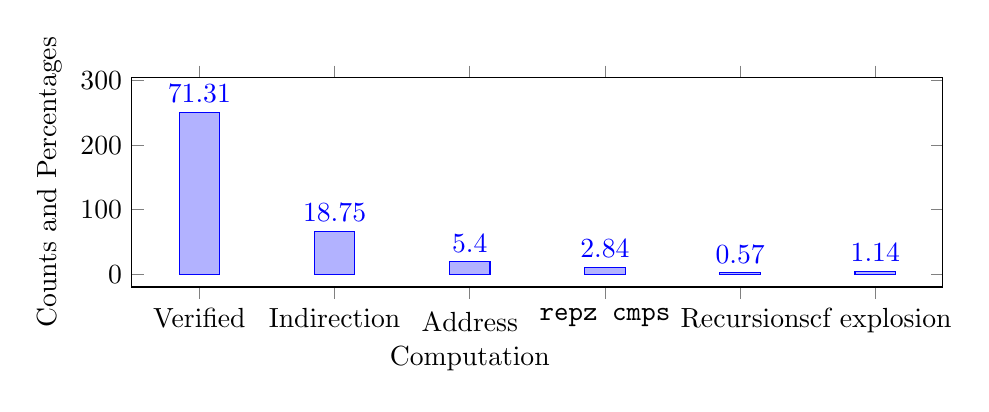
\begin{tikzpicture}
    \begin{axis}[
      width=0.98\linewidth,
      height=0.35\linewidth,
      ybar,
      ylabel=Counts and Percentages,
      bar width=0.3,
      nodes near coords, % causes build failure when combined with symbolic x coords
      point meta=y/3.52, % can't get \% shown right
      enlarge y limits={value=0.2, upper},
      ymin=-20,
      xticklabels={
        Verified,
        Indirection,
        \begin{tabular}{c}Address\\Computation\end{tabular},
        \texttt{repz cmps},
        Recursion,
        \acs{scf} explosion
      },
      xtick=data
    ]
    \addplot coordinates {
      (0, 251)
      (1, 66)
      (2, 19)
      (3, 10)
      (4, 2)
      (5, 4)
    };
    \end{axis}
  \end{tikzpicture}
  \caption{Analzyed Xen Functions Compared to Unverified Features}
  \label{fig:unverified}
\end{figure*}

This methodology is currently capable of dealing with \xenpercentage\
of the functions present in the aforementioned binaries (see \cref{fig:unverified}).
The supported features include (nested) loops,
subcalls, variable argument lists, jumps into other function bodies,
string instructions with the \texttt{rep} prefix, and \ac{simd} instructions.
There is no particular limit on function size.
The average number of instructions per function analyzed is 49.
Some of the functions analyzed have over 300 instructions and over 100 basic blocks.

There are five categories of features not currently supported.
The first and most common is \emph{indirection}, accounting for \SI{19}{\percent}.
\index{indirection}
Indirection involves a call or jump instruction
that loads the target address from a register or memory location
rather than using a static value.
Switch statements and certain uses of \texttt{goto}
are the most common causes of indirect jumps.
Indirect calls generally result from usage of function pointers.
For example, the \lstinline|main| functions of all three verified binaries
used switch statements in loops in the process of parsing command line options.
These statements introduced indirect branches.

The second category involves issues related to generating the \acp{mrr}.
This step requires solving linear arithmetic over symbolically computed addresses.
\index{linear arithmetic}
Sometimes, addresses are computed using a combination of arithmetic operators
\index{operator!arithmetic}
with bitwise logical operators.
\index{operator!bitwise}
In some of these cases, our translation to Z3 does not produce an answer.
\index{Z3}
As an example, function \texttt{qcow\_open}
uses the rotate-left function to compute an address.
As another example, function \texttt{AES\_set\_encrypt\_key}
produces addresses that are obtained via combinations of bit-shifting,
bit masking, and \texttt{xor}-ing.
For these cases, separation and enclosure relations cannot be generated.

The instruction \texttt{repz cmps} is currently not supported for technical reasons.
It is the assembly equivalent of the function \texttt{strncmp},
but instead writes its result to a flag.
Various other string-related instructions with the \texttt{rep} prefix are supported,
however.

Functions with \emph{recursion}, a minority in systems code, are also not supported.
Recursive stack frames are not well-suited to automation in this framework.
The two recursive functions encountered both perform file-system-like tasks.
Functions \lstinline|do_chmod| and \lstinline|do_ls| are similar to the permission-setting \lstinline|chmod| utility
and the directory-displaying \lstinline|ls|, respectively.

The final category is functions whose \ac{scf} explodes.
The issue occurs when the pattern in \cref{fig:ex_nonopt} shows up extensively
or when while loops have multiple entries.

\Cref{func-counts} provides an overview of the verification effort.
The table shows the absolute counts of functions verified
as well as the total number of instructions for those functions.
Alongside that information is the number of functions with loops
that were verified and how many manual lines of proof were required in total.
The vast majority of those manual proof lines were related to the loop count.
Meanwhile, a comparison with those functions not verified
can be found in \cref{fig:unverified}.

\section{Conclusion}
